\documentclass{article}

\usepackage{authblk}
\usepackage{amsmath}
\usepackage{tikz}
\usepackage{caption}
\usepackage{subcaption}
\usepackage{graphicx}
\usepackage{titlesec}
\usepackage{hyperref}

\graphicspath{ {./} }

\author{Aurora Zuoris \\ \normalsize{aurora.zuoris101@alu.ulpgc.es}}
\affil{Universidad de Las Palmas de Gran Canaria}
\title{Parallel matrix multiplication}

\begin{document}

\maketitle

\abstract {
As computational power continues to advance in the era of Moore's Law,
the focus has shifted from increasing individual core speeds to the proliferation of multicore architectures.
This paradigm shift increases the need for optimizing parallel algorithms,
particularly in the context of matrix multiplication.
}

\section{Introduction}

Implementing a parallel algorithm for matrix multiplication can be crucial as we are reaching the limit of how fast
a single CPU core can go, and thus more and more modern computers come with multiple cores, thus a sequential algorithm wouldn't
use the hardware most computers come with to the fullest.

\section{Implementations}

The source code can be found at the author's github profile\footnote{\url{https://github.com/Aurora2500/parallel-matrix-big-data}}

For this paper, two implementations will be done,
one naive implementation that ,
and the other implementation using tiled matrix multiplication.

Taking into consideration the equation of matrix multiplication:

\begin{equation*}
	c_{ij} = \sum_{k=1}^K a_{ik} \cdot b_{kj}
\end{equation*}

the naive implementation consists of dividing the resulting matrix into chunks and giving each thread different chunks.
This way, all the threads will need read access to both input matrices, and write only in their own chunk of the resulting matrix.
This is safe as concurrent reading of immutable data is safe, and each thread will only mutate their own assigned chunks of memory, so there
isn't any race conditions.

Tiled matrix multiplication on the other hand works by dividing up the matrix in blocks and then applying smaller matrix multiplication on these blocks,
aggregating them at the end by adding them all up.
While from a first point of view there isn't much of a reason for this implementation to be faster,
it does have a plethora of unique properties that makes it interesting and gives it some benefits in different environments, altough none of them
have to do with speedup directly, but rather with how the matrices can be split up and the number of memory access that's performed.


\section{Results}

\begin{figure}[h!]
	\centering
	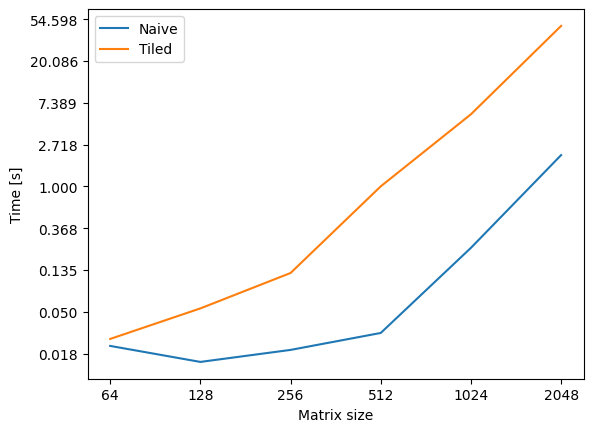
\includegraphics[width=0.8\textwidth]{result.png}
\end{figure}

Surprisingly, a simple naive implementation is faster than the tiled implementation. It should be noted that this benchmark was implemented on
the CPU, where the pros of the tiled implementation don't appear as strongly.

\section{Future work and conclusions}

For now it seems that a naive matrix multiplication algorithm is better, at least for computing on the CPU.
But it could be that tiled matrix multiplication is better for example on the GPU due to its memory access characteristics,
or on distributed programming given that it can be split up to do work using less memory from the factor matrices.

In the future it would be interesting to implement distributed algorithms as in these the tiled implementation is basically the only way
to do it feasibly for larger matrix sizes, as a smaller part of the original matrices is needed during each step of the computation.

\end{document}